\section{Pokazać, że grupa multiplikatywna ciała skończonego jest grupą cykliczną.}
\begin{theorem}
	Dla ciała skończonego \( \mathbb{F}_q \) istnieje taki element \( g \), że \( \mathbb{F}^{*}_q = \set{1, g, g^2, \text{\dots}} \).
\end{theorem}
\begin{proof}
	Oznaczmy \( n = \abs{\mathbb{F}^{*}_q} = q-1 \). Definiujemy zbiory:
	\[
		A_d = \set{a \in \mathbb{F}_q : a^d = 1}
	\]
	\[
		B_d = \set{a \in \mathbb{F}_q : a^d = 1, a^{d'} \neq 1 \text{ dla } d' < d}
	\]
	czyli \( B_d \) zawiera elementy, których rząd jest równy \( d \). Widać, że \( B_d \subseteq A_d \).

	Z twierdzenia Lagrange'a wynika, że \( B_d \) może być niepusty tylko dla \( d \) będącego dzielnikiem \( n \), a także \( \sum_{d \mid n} \abs{B_d} = n \), bo każdy element należy do któregoś \( B_d \). Chcemy pokazać, że \( B_n \neq \emptyset \), czyli istnieje element rzędu \( n \).

	Jeśli dla pewnego \( d \) zachodzi \( B_d \neq \emptyset \), to \( \abs{A_d} \geq d \), bo jeśli \( a^d = 1 \), to również \( (a^j)^d = 1 \) dla~\( 0 \leq j < d \). Z drugiej strony, \( \abs{A_d} \leq d \), bo wielomian \( X^d-1 \) może mieć co najwyżej \( d \) pierwiastków. Zatem jeśli istnieje element rzędu \( d \), to \( \abs{A_d} = d \).
	Wtedy \( \abs{B_d} = \varphi(d) \) -- na ćwiczeniach udowodniliśmy, że jeśli istnieje jakiś generator, to można znaleźć \( \varphi(d) \) generatorów.
	Podsumowując, dla każdego \( d \) zachodzi jedna z dwóch możliwości:
	\begin{itemize}
		\item \( \abs{B_d} = 0 \)
		\item \( \abs{B_d} = \varphi(d) \)
	\end{itemize}
	Wynika stąd, że
	\[
		n = \sum_{d \mid n} \abs{B_d} \leq \sum_{d \mid n} \varphi(d),
	\]
	przy czym jeśli chociaż jedno \( d \) ma \( B_d = \emptyset \), to nierówność jest ostra.

	Wiemy jednak, że \( \sum_{d \mid n} \varphi(d) = n \), ponieważ możemy rozważyć wszystkie \( n \) ułamków właściwych postaci \( \frac{k}{n} \) dla \( 1 \leq k \leq n \).
	Po skróceniu mają postać \( \frac{k'}{d} \), gdzie \( d \mid n \) oraz \( k' \) jest względnie pierwsze z \( d \), więc dokładnie \( \varphi(d) \) ułamków ma taki mianownik. To dowodzi równości.

	Zatem nierówność nie może być ostra i zachodzi \( B_d \neq \emptyset \) dla każdego \( d \mid n \), w szczególności istnieje element rzędu \( n \).
\end{proof}


\section{Opisać algorytm ,,ro'' Pollarda na faktoryzację.}
\label{C:rho_factorization}
Celem jest rozłożyć na czynniki liczbę złożoną \( n \). Załóżmy, że \( p \leq \sqrt{n} \) jest jakimś jej dzielnikiem pierwszym.
Wybieramy łatwo obliczalną funkcję, niech to będzie \( f(x) = x^2 + 1 \). Chcemy zbadać ciąg \( x_0 = 2 \), \( x_k = f(x_{k-1}) \).
Zakładamy, że wartości będą się rozkładały równomiernie modulo \( n \). Ciąg powinien się zapętlić po około \( \sqrt{n} \) krokach. Przypuszczamy jednak, że uda się to zaobserwować już wcześniej, po \( \sqrt{p} \) krokach.

Jeśli znajdzie się \( x_i = x_j \pmod{p} \), to \( \gcd(x_i - x_j, n) \) powinno być nietrywialnym dzielnikiem \( n \), ponieważ wykonaliśmy zbyt mało kroków, żeby \( n \mid (x_i - x_j) \).
Jeśli powstanie cykl modulo \( p \) o długości \( s \), to taka sytuacja będzie się powtarzać dla dowolnych \( x_i, \ x_{i+s} \). Zamiast co krok sprawdzać dla wszystkich \( x_{i<j} \) przystawania do \( x_j \),
wykorzystujemy metodę Floyda lub Brenta, żeby wykryć długość cyklu.
\begin{greyframe}
    Algorytm Pollarda (wariant Floyda):
    \begin{enumerate}
        \item Jeśli \( 2 \mid n \), zwróć 2.
        \item Zdefiniuj \( x = x_0, y = x_0, d = 1 \).
        \item Dopóki \( d \) jest trywialny:
        \begin{enumerate}
            \item Oblicz \( x = f(x) \pmod{n} \), \( y = f(f(y)) \pmod{n} \).
            \item Oblicz \( d = \gcd(x-y, n) \).
        \end{enumerate}
        \item Jeśli \( d \neq n \), zwróć \( d \).
        \item Powtórz procedurę od kroku 2, losując nowe \( x_0 \) oraz funkcję \( f \).
    \end{enumerate}
\end{greyframe}
Zapętlenie oraz wyłapanie tego wymaga w oczekiwaniu około \( \sqrt{p} + s \leq 2\sqrt{p} = \bigO(\sqrt[4]{n}) \) kroków. Jeśli algorytm kończy się powodzeniem, po tylu krokach \( \gcd(x_i - y_i, n )\) jest dzielnikiem \( n \).
Są jednak dwa scenariusze niepowodzenia:
\begin{itemize}
    \item Wyrazy ciągu mogą nie powtórzyć się wystarczająco szybko \\
    -- przerywamy procedurę po \( 5\sqrt[4]{n} \) krokach.
    \item Ciąg pętli się modulo \( p \) i modulo \( n \), czyli \( \gcd(x_i - y_i, n) = n \) \\
    -- przerywamy od razu.
\end{itemize}

\subsection{Metoda Floyda}
Pomysł polega na tym, żeby w każdym kroku sprawdzać tylko wartość \( \gcd(x_{2k} - x_k, n) \), ponieważ te dwa wyrazy przystają do siebie modulo \( p \), kiedy \( k \) jest wielokrotnością \( s \).
Ciąg \( x_{2k} \) definiujemy jako \( x_{2k} = y_k = f(f(y_{k-1})) \), \( y_0 = x_0 \), unikając w ten sposób przechowywania wielu poprzednich wartości.

\subsection{Metoda Brenta}
Sprawdzamy, czy ciąg się zapętlił, wykonując kolejno \( K = 1, 2, 4, 8, \dots \) kroków. Jeśli w \( K \) krokach wyraz ciągu powtórzy się modulo \( p \), to udało się znaleźć wspólny dzielnik. Jeśli nie, to powtarzamy próbę dla kolejnego \( K \), zaczynając od miejsca, w którym skończyliśmy.

Ten wariant ma nieco lepszą stałą niż metoda Floyda.


\section{Opisać algorytm sita kwadratowego.}
\subsection{Faktoryzacja przez liczby \( B \)-gładkie}
\begin{definition}
	Dla ustalonego \( B \) liczba \( B \)-gładka to taka, której wszystkie pierwsze dzielniki są mniejsze od \( B \).
\end{definition}

Celem jest rozłożyć \( N \) na czynniki pierwsze. Ustalamy pewne \( a_1, \dots, a_k \), po czym obliczamy \( b_i = a_i^2 \pmod{N} \). Chcemy wybrać taki podzbiór \(b_i \), żeby iloczyn jego elementów był pełnym kwadratem.

\begin{lemma}
	Niech \( \set{p_1, \dots, p_{s}} \) będzie zbiorem liczb pierwszych mniejszych od \( B \). W każdym zbiorze liczb \( B \)-gładkich o liczności większej od \( s \) istnieje podzbiór, którego iloczyn jest kwadratem.
\end{lemma}
\begin{proof}
	Niech \( \set{x_1, \dots, x_k} \) dla \( k > s \) będą liczbami \( B \)-gładkimi. Rozkładamy każdą z nich na czynniki pierwsze:
	\[
		x_i = p_1^{\alpha_{1, i}} \cdots p_s^{\alpha_{s, i}}
	\]
	a następnie przypisujemy jej wektor:
	\[
		v_i = (\alpha_{1, i}, \dots, \alpha_{s, i}) \mod 2
	\]
	Jeśli dla \( \set{x_1, \dots, x_k} \) każdy czynnik \( p_i \) występuję parzyście wiele razy, czyli \( v_1 \oplus \ldots \oplus v_k = 0 \), jest to poszukiwany podzbiór.
	Skoro \( k > s \), to wektory \( v_1, \dots, v_k \) są liniowo zależne w \( \integer_2^{s} \), więc taki podzbiór musi istnieć i można go znaleźć za pomocą eliminacji Gaussa w \( \bigO(s^3) \).
\end{proof}
Powyższą teorię można przekształcić na praktyczną metodę faktoryzacji liczby \( N \).
\begin{greyframe}
	Algorytm faktoryzacji:
	\begin{enumerate}
		\item Znajdź takie \( a_1, \dots, a_k \), że \( b_i = a_i^2 \pmod{N} \) jest \( B \)-gładkie.
		\item Dla każdego \( b_i \) wyznacz wektor \( v_i \).
		\item Znajdź taki podzbiór \( I \subseteq \set{1, \dots, k} \), że wektory \( v_{i \in I} \) są liniowo zależne.
		\item Przypisz \( u = \prod_{i \in I} a_i \pmod{N} \) oraz \( v = \sqrt{\prod_{i \in I}\; b_i} \pmod{N} \).
		\item Jeśli \( u \neq \pm v \), to \( \gcd(u + v, N) \) jest nietrywialnym dzielnikiem \( N \), \\ ponieważ \( u^2 = v^2 \pmod{N} \).
		\item Jeśli \( u = \pm v \), to powtórz procedurę.
	\end{enumerate}
\end{greyframe}
Krok 1. jest na razie czarną skrzynką, ale można za nią podstawić algorytm sita kwadratowego.

\subsection{Sito kwadratowe}
Poszukiwane liczby \( a_i \) muszą być większe od \( \sqrt{N} \), inaczej \( u = v \). Sprawdzamy więc po kolei dla potencjalnych kandydatów, czy reszty są \( B \)-gładkie.
Dla ustalonego \( K \) oraz \( i \in \set{0, \dots, K-1} \) definiujemy:
\[ X[i] = \ceil{\sqrt{N}} + i \]
\[ Y[i] = X[i]^2 \pmod{N} = \pars{\ceil{\sqrt{N}} + i}^2 - N \]
Trzeba rozłożyć liczby \( Y[i] \) na czynniki -- najlepiej wszystkie na raz, poniższym algorytmem.
\begin{greyframe}
	Algorytm sita kwadratowego:
	\begin{enumerate}
		\item Dla każdego \( p < B \):
		      \begin{enumerate}
			      \item Usuń ze zbioru \( \set{p_1, \dots, p_s} \) te liczby, dla których \( X[j]^2 \neq N \pmod{p} \), \\ czyli \( N \) nie jest resztą kwadratową modulo \( p \).
			      \item Algorytmem Tonellego-Shanksa znajdź rozwiązanie \( x = \pm k \) równania \\ \( x = N \pmod{p} \).
			      \item Podziel przez \( p \) wszystkie \( Y[i] \), dla których \( X[j] = \pm k \pmod{p} \).
		      \end{enumerate}
		\item Jeśli \( Y[i] \) zmaleje do 1, to początkowo musiało być liczbą \( B \)-gładką.
	\end{enumerate}
\end{greyframe}
W ramach dodatkowego usprawnienie algorytmu, możemy uniknąć dzielenia dużych liczb. Zamiast wartości \( Y[i] \) przechowujemy \( Z[i] = \log Y[i] \).
Wtedy operację \( \frac{Y[i]}{p} \) zastępujemy działaniem \( Z[i] - \log p \). Warunkiem \( B \)-gładkości jest (prawie) wyzerowanie się \( Z[i] \).
Problemem może być występowanie czynników \( Y[i] \) z potęgą \( \alpha > 1 \). Należy wykryć od razu liczby \( Y[i] \) podzielne przez \( p^{\alpha} \) dla każdego możliwego \( \alpha \), stosując tę samą metodę.

Przy optymalnym wyborze parametrów, czyli \( B, \ K \) rzędu \( e^{\sqrt{\ln N \ln\ln N}} \), złożoność algorytmu wynosi \( \bigO(e^{(1 + {\scriptscriptstyle\mathcal{O}}(1))\sqrt{\ln N \ln\ln N}}) \), czyli jest podwykładnicza.

\subsection{Metoda Multi Polynomial Quadratic Sieve (MPQS)}
Algorytm sita kwadratowego można zrównoleglić, używając wielu różnych wielomianów postaci \( (A \cdot X + B)^2 - N \) zamiast \( X^2 - N \).


\section{Opisać algorytm ,,ro'' Pollarda na logarytm dyskretny.}
\externaldocument{chapters/B/main}
Trudno na ten moment poprawić pierwiastkową złożoność czasową algorytmu Baby-Step-Giant-Step, można jednak zmniejszyć użycie pamięci -- w algorytmie ,,ro'' Pollarda wystarcza \( \bigO(1) \).

Główny pomysł polega na tym, żeby generować pary postaci \( a^{\alpha_i} \cdot b^{\beta_i} \), dla różnych \( \alpha_i \) oraz \( \beta_i \), aż wystąpi kolizja.

Jeśli \( a^{\alpha_i} \cdot b^{\beta_i} = a^{\alpha_j} \cdot b^{\beta_j} \), to \( a^{\alpha_i - \alpha_j} = b^{\beta_j - \beta_i} \). Wystarczy więc znaleźć \( \beta^{*} = (\beta_j - \beta_i)^{-1} \) modulo \( \abs{G} \) i otrzymamy \( a^{\beta^{*} (\alpha_i - \alpha_j)} = b \).

Ciąg \( (\alpha_i, \beta_i) \) definiujemy, losując wartości początkowe \( (\alpha_0, \beta_0) \), a kolejne obliczając za pomocą jakiejś deterministycznej funkcji \( f \), która zapewni pseudolosowość wyników.
Jeśli w pewnym momencie \( (\alpha_i, \beta_i) = (\alpha_j, \beta_j) \), to tak już zostaje, czyli ciąg wpada w pętlę literki ,,ro''. Drugi ciąg można zdefiniować za pomocą metody Floyda (patrz: pytanie~\ref{C:rho_factorization}):
\[ (\alpha'_{i+1}, \beta'_{i+1}) = f(f(\alpha'_i, \beta'_i)) \]
W każdym kroku sprawdzamy, czy \( (\alpha_i, \beta_i) = (\alpha'_i, \beta'_i) \). Jeśli ciągi są losowe, to kolizja wystąpi w oczekiwaniu po \( \sqrt{\abs{G}} \) krokach.

Pozostaje uszczegółowić wybór funkcji \( f \). Powinna ona rozrzucać wartości ciągu możliwie przypadkowo wśród elementów \( G \). Technika stosowana w praktyce jest następująca:
\begin{itemize}
	\onehalfspacing
	\item Wybieramy małą liczbę naturalną \( n \).
	\item Wybieramy funkcję haszującą \( h \), która parze liczb całkowitych \( (\alpha, \beta) \) przyporządkowuje liczbę ze zbioru \( \set{1, 2, \dots, n} \).
	\item Losujemy liczby naturalne \( x_1, \dots, x_n \) oraz \( y_1, \dots, y_n \).
	\item Definiujemy \( f(\alpha, \beta) = (\alpha + x_s, \beta + y_s) \), gdzie \( s = h(\alpha, \beta) \).
\end{itemize}

Algorytm ,,ro'' działa w oczekiwanym czasie \( \bigO\pars{\sqrt{\abs{G}}} \) i stałej pamięci.

\section{Opisać algorytm Pohliga-Hellmana.}
Algorytm jest heurystyką, korzystającą z faktu, że rząd grupy często jest liczbą złożoną. Mając daną grupę \( G = \langle g \rangle \) o \( n \) elementach oraz \( b \in G \), chcemy znaleźć \( x \), rozwiązanie równania \( g^x = b \).
\begin{greyframe}
	Algorytm Pohliga-Hellmana:
	\begin{enumerate}
		\item Jeśli \( n \) jest liczbą pierwszą, to wyznacz \( x \) algorytmem Baby-Step-Giant-Step \\ \( \rightarrow \bigO(\sqrt{n}) \).
		\item Jeśli \( n = p^k \), gdzie \( p \) jest pierwsze oraz \( k > 1 \), to:
		      \begin{enumerate}
			      \item Zapisz (nieznany jeszcze) \( x \) w systemie o podstawie \( p \) jako
			            \[
				            x = x_0 + x_1 \cdot p + \ldots + x_{k-1} \cdot p^{k-1}
			            \]
			      \item Na podstawie równania:
			            \[
				            \pars{g^x}^{p^{k-1}} = \pars{g^{x_0}}^{p^{k-1}} = b^{p^{k-1}},
			            \]
			            zdefiniuj \( h = g^{p^{k-1}} \) o rzędzie \( p \).
			      \item Rozwiąż równanie postaci \( h^{x_0} = b^{p^{k-1}} \) dla \( x_0 \), czyli oblicz logarytm dyskretny w~grupie \( \set{1, h, h^2, \ldots, h^{p-1}} \) \( \rightarrow \bigO(\sqrt{p}) \) (przypadek 1).
			      \item Sprowadź równanie do postaci:
			            \[
				            g^{x_1 \cdot p + \ldots + x_{k-1} \cdot p^{k-1}} = b \cdot g^{-x_0}
			            \]
			            Po podniesieniu równania do potęgi \( p^{k-2} \), oblicz \( x_1 \), rozwiązując \( h^{x_1} = \pars{b \cdot g^{-x_0}}^{p^{k-2}} \).
		      \end{enumerate}
		      Powtórz procedurę dla \( x_0, x_1, \ldots, x_{k-1} \) \( \rightarrow \bigO(k \sqrt{p}) \).
		\item Jeśli \( n  = q_1 \cdot q_2 \), gdzie \( \gcd(q_1, q_2) = 1 \), to:
		      \begin{enumerate}
			      \item Zapisz \( x \) jako \( x = u_1 \cdot q_1 + r_1 \).
			      \item Podnieś równanie do potęgi \( q_2\):
			            \[
				            g^{u_1n + r_1q_2} = b^{q_2}
			            \]
			            Przy \( g^n = 1 \) daje to \( g^{r_1 q_2} = b^{q_2} \), czyli \( h = g^{q_2} \) ma rząd \( q_1 \).
			      \item Oblicz \( r_1 \) takie, że \( x = r_1 \pmod{q_1} \), rekurencyjnie na grupie \( H = \langle h \rangle \).
			      \item Analogicznie, oblicz \( r_2 \) takie, że \( x = r_2 \pmod{q_2} \).
			      \item Z CRT wyznacz \( x \), rozwiązanie układu kongruencji \( x = u_i \cdot q_i + r_i \).
		      \end{enumerate}
		      Jeżeli \( n = p_1^{\alpha_1} \cdot \ldots \cdot p_s^{\alpha^s} \), to rekurencyjnie wywołaj przypadek 2 dla każdego \( p_i^{\alpha_i} \) \( \rightarrow \bigO(\sum_i \alpha_i \sqrt{p_i}) \leq \bigO(\log n \cdot \sqrt{\max{p_i}}) \), bo \( \alpha_i \leq \log n \).
	\end{enumerate}
\end{greyframe}

Algorytm działa szybko, jeśli rząd grupy ma tylko małe dzielniki. Zazwyczaj radzi sobie też z grupą \( GF(p^k) \) ciała skończonego, ponieważ rząd grupy \( p^k - 1 \) najczęściej jest liczbą złożoną.
Rozsądnym wyborem jest \( \integer^{*}_p \) dla \( p = 2q + 1 \), gdzie \( p, \ q \) są pierwsze (liczby pierwsze Sophie Germain).


\newpage
\section{Opisać algorytm rachunku indeksów.}
Rachunek indeksów to obecnie najlepszy znany algorytm na logarytm dyskretny w \( \integer_p \).

Działając w grupie \( \integer_p \) o znanym generatorze \( g \), dla \( g^x = b \) chcemy znaleźć \( x = \log b \). Taki logarytm zachowuje własności zwykłego logarytmu.

\textbf{Faza I:} \\
Ustalamy zbiór małych liczby pierwszych \( Q = \{q_1, \dots, q_r\} \) -- bazę czynników.
Wybieramy lub losujemy \( k \), tak żeby uzyskać \( r \) różnych liczb, dla których \( g^k \pmod{p} \) rozkłada się na czynniki z bazy \( Q \). W ten sposób otrzymujemy \( r \) równań postaci:
\[
    g^k = q_1^{\beta_1} \cdot \ldots \cdot q_r^{\beta_r} \pmod{p},
\]
\[
    \text{czyli } k = \beta_1 \cdot \log q_1 + \ldots + \beta_r \cdot \log q_r \pmod{p - 1}
\]

\textbf{Faza II:} \\
Znając wszystkie \( \beta_i \) oraz \( k \), chcemy rozwiązać układ równań:
\[
    k^{(1)} = \beta_1^{(1)} \cdot \log q_1 + \ldots + \beta_r^{(1)} \cdot \log q_r
\]
\[
    \cdots
\]
\[
    k^{(r)} = \beta_1^{(r)} \cdot \log q_1 + \ldots + \beta_r^{(r)} \cdot \log q_r
\]
z niewiadomymi \( \log q_i \). Możemy wykorzystać do tego metody algebry liniowej z dokładnością do jednej trudności -- operacje są modulo \( p-1 \), które nie jest pierwsze, więc niekoniecznie da się policzyć odwrotność względem mnożenia.
Jako wynik otrzymujemy logarytmy dyskretny liczb \( q_1, \dots, q_r \).

\textbf{Faza III:} \\
Żeby znaleźć \( \log b \), próbujemy wygenerować jakąkolwiek liczbę postaci \( b^u \cdot g^v \), która jest gładka modulo \( p \). Wystarczy przyjąć \( u = 1 \) i losować \( v \) do skutku. Z równości
\[ b^u \cdot g^v = q_1^{\gamma_1} \cdot \ldots \cdot q_r^{\gamma_r} \]
ostatecznie wynika:
\[ x = \log b = u^{-1} \cdot (\gamma_1 \cdot \log q_1 + \ldots + \gamma_r \cdot \log q_r - v) \]

Oczekiwana złożoność algorytmu to \( e^{(\sqrt{2}+\bigO(1))\sqrt{\ln n \ln\ln n}} \), czyli podwykładnicza. Metoda rachunku indeksów daje się uogólnić na ciała skończone \( \integer_p[X]/(w) \), gdzie \( w \) jest pewnym wielomianem. Wtedy baza czynników, zamiast liczb pierwszych, zawiera nierozkładalne wielomiany małych stopni.

\subsection{Atak Logjam}
Rachunek indeksów, jeśli stosowany w sposób leniwy, ma słaby punkt -- fazy I i II są niezależne od wejściowego elementu \( b \), co gorsza można je łatwo zrównoleglić.
Żeby rozszyfrować ciąg informacji, dla których zawsze używana była ta sama liczba pierwsza \( p \), wystarczy wykonać fazy I i~II tylko raz, a faza III jest już bardzo szybka.


\section{Opisać ideę algorytmu Sch{\"o}nhage-Strassena.}
\subsection{Teoretyczna Transformata Numeryczna (NTT)}
Transformata NTT (\textit{Number Theoretic Transform}) jest wersją FFT, która nie używa liczb rzeczywistych -- zamiast nad \( \real \), obliczenia są wykonywane nad \( \integer_p \).
Wzory rekurencyjne i własność wzajemnej odwrotności DFT i IDFT przenoszą się na pierścień \( \integer_p \). Jedynym warunkiem jest, żeby \( \omega \in \integer_p \) spełniało \( \omega^n = 1 \) oraz  \( \omega^{\frac{n}{2}} = -1 \), czyli żeby \( \omega \) było rzędu \( n \).
Z twierdzenia Lagrange'a oraz faktu, że \( \integer_p \) jest cykliczna wiemy, że taki element istnieje, jeśli \( n \mid (p - 1) \). Algorytm FFT modulo \( p \) (czyli właśnie NTT) działa dla \( p \) postaci \( q \cdot n + 1 \).

\begin{greyframe}
    Splatanie ciągów \( A = (a_0, a_1, \ldots, a_n) \) i \( B = (b_0, b_1, \ldots, b_n) \):
    \begin{enumerate}
        \item Znajdź \( p \) postaci \( q \cdot n + 1 \), gdzie \( q \) jest niedużą liczbą pierwszą -- można wylosować i sprawdzić pierwszość lub szukać po kolei.
        \item Znajdź generator \( g \) grupy \( \integer^{*}_p \) -- generatorów jest \( \varphi(q \cdot n) = (q - 1) \cdot \frac{n}{2} \), więc losowanie zadziała.
        Generator musi spełniać \( g^{\frac{p-1}{2}} \neq 1 \pmod{p} \) oraz \( g^{\frac{p-1}{q}} \neq 1 \pmod{p} \).
        \item Ustal \( \omega = g^q \) rzędu \( n \) i oblicz splot za pomocą NTT.
    \end{enumerate}
\end{greyframe}
Można wybrać na tyle duże \( p \), żeby modulo nie miało wpływu na wynik. Przy mnożeniu liczb binarnych wystarczy \( p > n \).

\subsection{Algorytm Sch{\"o}nhage-Strassena}
Algorytm służy do mnożenia dużych liczb w zapisie binarnym. Ponieważ daje on zysk praktyczny dopiero w przypadku \emph{naprawdę} dużych liczb, musi radzić sobie z problemami wynikającymi z długości ich zapisu.

Pierwszym z wyzwań jest wybór pierścienia do obliczeń -- jeśli liczba \( p \) jest duże, to operacje w \( \integer_p \) nie są jednostkowe.

Liczba \( p \) nie musi być pierwsza, wystarczy nam względna pierwszość z \( n \), (potrzebne jest dzielenie przez \( n \)) i musi istnieć element \( \omega \) rzędu \( n \) modulo \( p \).
Te warunki spełniają \( p = 2^m + 1 \), \\ \( \omega = 2^{\alpha} \) takie, żeby \( \omega^n = 1 \pmod{p} \). Sprytny dobór liczb upraszcza obliczenia:
\begin{itemize}
    \item branie reszty modulo \( p \) -- zauważamy, że \( 2^m = p - 1 = -1 \pmod{p} \), więc możemy podzielić liczbę na \( m \)-cyfrowe fragmenty i dodać je z naprzemiennymi znakami:
    \[
        101001110_2 \pmod{2^3 + 1} = 101_2 - 001_2 + 110_2 \pmod{2^3 + 1},
    \]
    \item mnożenie przez \( \omega = 2^{\alpha} \) -- dopisujemy zera na końcu liczby binarnej i wyciągamy resztę modulo \( p \),
    \item dzielenie przez \( \omega = 2^{\alpha} \) -- mnożymy przez \( \omega^{-1} = -2^{m-\alpha} \), czyli też potęgę 2.
    \item mnożenie dwóch liczb w \( \integer_p \) -- nadal trudne, ale wykonujemy je niewiele razy i można sobie z nim poradzić rekurencją na liczbach o długości \( m \),
\end{itemize}

Algorytm Sch{\"o}nhage-Strassena służy do obliczania iloczynu \( N \)-bitowych liczb \( A \), \( B \) modulo \( p = 2^N + 1 \).
Jeśli chce się otrzymać wynik pełny (nie modulo), wystarczy przyjąć \( N \) większe od sumy długości liczb na wejściu. Zakładamy, że \( N \) jest potęgą 2. Algorym działa rekurencyjnie, sprowadzając iloczyn \( A \) i \( B \) do splotu wielomianów w mniejszym pierścieniu.

\begin{greyframe}
    Algorytm fastmul(\( A, B, N \)):
    \begin{enumerate}
        \item Rozbijamy liczby \( A \) i \( B \) na fragmenty o długości około \( \sqrt{N} \), czyli na \( t \) binarnych liczb \( b \)-cyfrowych. Liczby \( t, \ b \) powinny być potęgami dwójki wielkości mniej więcej \( \sqrt{N} \).
        \[
            A = u_0 + u_1 \cdot 2^b + u_2 \cdot 2^{2b} + \ldots + u_{t-1} \cdot  2^{(t-1)b}
        \]
        \[
            B = v_0 + v_1 \cdot 2^b + v_2 \cdot 2^{2b} + \ldots + v_{t-1} \cdot 2^{(t-1)b}
        \]
        Zadanie sprowadza się do pomnożenia dwóch liczb \( t \)-cyfrowych w systemie o podstawie \( 2^b \).

        \item Wykonujemy algorytm NTT w pierścieniu \( \integer_p \) dla \( p = 2^{b'} + 1 \). Wymaga to obliczenia \( 2t \) iloczynów modulo \( 2^{b'} + 1 \) rekurencyjnie.
    \end{enumerate}
\end{greyframe}

W punkcie 2 splatamy liczby w pierścieniu \( \integer_p \) dla \( p = 2^{b'} + 1 \), gdzie \( b' \approx 2b + \log t \) oraz \( t \mid b' \). Bierze się to stąd, że wynik splotu nie przekracza \( p \), czyli \( p > t \cdot \pars{2^b}^2 \), więc \( b' \geq 2b + \log t \).
Podzielność \( t \mid b' \) jest ważna, żeby rząd \( \omega = 2^{\frac{2b'}{t}} \) był równy \( t \), czyli \( \omega^{\frac{t}{2}} = 2^{b'} = -1 \pmod{p} \).

Algorytm można opisać ogólnym równaniem
\[
    T(n) = 2 \sqrt{n} \cdot T(\alpha \sqrt{n}) + \Theta(n \log n)
\]
dla pewnego całkowitego \( \alpha \).

Sprowadzamy mnożenie dwóch liczb \( N \)-bitowych do około \( 2\sqrt{N} \) mnożeń liczb o długości \( 4\sqrt{N} \), co daje złożoność \( \bigO(N \log^2 N) \).
Poprawienie jej do \( \bigO(N \log N \log \log N) \) wymaga zmniejszenia stałych \( (2, 4) \rightarrow (1, 2) \) technicznymi sztuczkami.
        
W praktyce rekursja jest płytka, ponieważ dla \( N < 10^3 \) lepiej użyć prostszych algorytmów, na przykład Tooma-Cooka albo nawet kwadratowego mnożenia.


\section{Opisać algorytm Schreiera-Simsa.}
\begin{definition}
    \textbf{Grupa permutacji} to zbiór \( S_n \) z działaniem składania permutacji.
\end{definition}

\begin{definition}
    \textbf{Stabilizatorem} \( i \) w grupie permutacji \( A \) jest zbiór \( A_i = \set{\pi \in A : \pi(i) = i} \).
\end{definition}

\begin{definition}
    \textbf{Orbitą} \( i \) w grupie permutacji \( A \) jest zbiór \(O_i = \set{\pi(i) : \pi \in A}\).
\end{definition}

Dla danego zbioru permutacji \(\Sigma = \set{\sigma_1, \sigma_2, \ldots, \sigma_k} \subset S_n\) chcemy określić, ile elementów ma grupa \(A \subseteq S_n\) generowana przez \(\Sigma\).

Korzystamy z następującego twierdzenia:
\begin{theorem}
    \( \abs{A} = \abs{A_1} \cdot \abs{O_1} \)
\end{theorem}
\begin{proof}
    Dzielimy grupę \( A \) na podzbiory \( B_1, \ldots, B_n \) zdefiniowane jako:
    \[
        B_x = \set{\pi \in A : \pi(1) = x}
    \]
    Zbiór \( B_x \) jest niepusty, jeśli \( x \in O_1 \), czyli istnieje permutacja \( \pi \in A \) taka, że \(\pi_x(1) = x\).
    Zatem odwzorowanie z \( A_1 \) do \( B_x \):
    \[
        \zeta \mapsto \pi_x \circ \zeta
    \]
    jest bijekcją i każdy niepusty zbiór \( B_x \) jest równoliczny z \( A_1 \). Stąd otrzymujemy:
    \[
        \abs{A} = \abs{B_1} + \ldots + \abs{B_n} = \abs{A_1} \cdot \abs{O_1},
    \]
    co było do pokazania.
\end{proof}

Z twierdzenia wynika schemat algorytmu:
\begin{greyframe}
    \begin{enumerate}
        \item Znajdź zbiór \( O_1 \).
        \item Utwórz zbiór \( \Sigma' \subseteq \Sigma \), który generuje \( A_1 \).
        \item Rekurencyjnie wyznacz \(\abs{A_1}\).
        \item Oblicz \(\abs{A} = \abs{O_1} \cdot \abs{A_1}\).
    \end{enumerate}
\end{greyframe}

\newpage
\subsubsection*{Jak wyznaczyć orbitę \(O_1\)?}
\begin{greyframe}
    \begin{enumerate}
        \item Utwórz graf \( G=(\set{1, \ldots, n}, E) \), gdzie \( E = \set{(x, \sigma_i(x)) : x \in V, \ \sigma_i \in \Sigma } \).
        \item Wyznacz \( O_1 \), czyli elementy osiągalne z \( 1 \), na przykład BFSem.
        \item Dla każdego \( x \in O_1 \) zapamiętaj \( \pi_x \in A \) taką, że \( \pi_x(1) = x \). \\
        Permutacja \(\pi_x\) jest złożeniem generatorów na ścieżce od \( 1 \) do \( x \).
    \end{enumerate}
\end{greyframe}

\subsubsection*{Jak wyznaczyć zbiór \(\Sigma'\) generujący \(A_1\)?}
Dla \(\sigma_i \in \Sigma\) oraz \(x \in \{1, 2, \ldots, n\}\) konstruujemy:
\[
    \tau_{i,x} = \pi_{\sigma_i(x)}^{-1} \circ \sigma_i \circ \pi_x
\]
Permutacja \(\tau_{i,x}\) działa następująco:
\[
    1 \xrightarrow{\pi_x} x \xrightarrow{\sigma_i} \sigma_i(x) \xrightarrow{\pi_{\sigma_i(x)}^{-1}} 1,
\]
czyli \(\tau_{i,x} \in A_1\).

\begin{lemma}[Schreiera]
    Zbiór \( \Sigma' = \set{\tau_{i,x} : 1 \leq i \leq k, \ 1 \leq x \leq n} \) generuje \( A_1 \).
\end{lemma}
\begin{proof}
    Dowolna permutacja \(\zeta \in A_1\) musi być iloczynem generatorów:
    \[
        \zeta = \sigma_s \circ \sigma_{s-1} \circ \ldots \circ \sigma_2 \circ \sigma_1
    \]
    Ustalamy \(y_j = (\sigma_j \circ \ldots \circ \sigma_1)(1)\), dla \(j = 1, 2, \ldots, s\) i dodajemy \(\pi_{y_j} \circ \pi_{y_j}^{-1}\) między każde \(\sigma_j\) i \(\sigma_{j+1}\):
    \[
        \zeta = \sigma_s \circ \pi_{y_{s-1}} \circ \pi_{y_{s-1}}^{-1} \circ \sigma_{s-1} \circ \pi_{y_{s-2}} \circ \pi_{y_{s-2}}^{-1} \circ \ldots \circ \sigma_2 \circ \pi_{y_1} \circ \pi_{y_1}^{-1} \circ \sigma_1
    \]
    Ponieważ \(\pi_1 = \text{id}\), otrzymujemy:
    \[
        \zeta = (\pi_1^{-1} \circ \sigma_s \circ \pi_{y_{s-1}}) \circ (\pi_{y_{s-1}}^{-1} \circ \sigma_{s-1} \circ \pi_{y_{s-2}}) \circ \ldots \circ (\pi_{y_1}^{-1} \circ \sigma_1 \circ \pi_1)
    \]
    Udało się wygenerować permutację \(\zeta\) jako złożenie generatorów z \(\Sigma'\).
\end{proof}
Konstrukcja zbioru \( \Sigma' \) jest poprawna, ale w rekurencji jego rozmiar może dojść do \( n! \), ponieważ \( \abs{\Sigma'} \approx n \cdot \abs{\Sigma} \).
Do kontroli nad tym służy filtr Simsa.

\newpage
\subsection{Filtr Simsa}
\begin{theorem}
    Dla dowolnego zbioru \( P \subseteq S_n \) istnieje zbiór \( Q \subseteq S_n \) taki, że podgrupy generowane przez \(P\) i \(Q\) są równe oraz \( \abs{Q} \leq \frac{n(n-1)}{2} \).
\end{theorem}
Dowód twierdzenia jest algorytmizowalny: \\
Dzielimy permutacje na klasy -- permutacja \(\zeta \neq \text{id}\) jest klasy \((i, j)\), jeśli:
\[
    \zeta(1) = 1, \zeta(2) = 2, \ldots, \zeta(i - 1) = i - 1,
\]
\[
    \zeta(i) = j > i.
\]
Chcemy, żeby w \( Q \) był co najwyżej jeden element z każdej klasy, ponieważ to gwarantuje, że \( \abs{Q} \leq \frac{n(n-1)}{2} \).

Zaczynając od \(Q = \emptyset\), przekładamy permutacje z \(P\) do \(Q\), utrzymując niezmienniki, że grupa generowana przez \( P \cup Q \) nie zmienia się i w \( Q \) jest co najwyżej jeden element każdej klasy.

Dla każdego elementu \(\zeta \in P\) klasy \((i, j)\):
\begin{enumerate}
    \item Jeśli w \(Q\) nie ma nic klasy \((i, j)\), przekładamy \(\zeta\) do \(Q\).
    \item Jeśli w \(Q\) jest element \(\varphi\) klasy \((i, j)\), zastępujemy \(\zeta\) przez \(\zeta' = \varphi^{-1} \circ \zeta\) i powtarzamy.
\end{enumerate}
Procedura zachowuje niezmienniki, ponieważ \(\zeta = \varphi \circ \zeta'\), więc zbiór generowany przez \(P \cup Q\) pozostaje taki sam.
Zmienia się natomiast klasa elementu, ponieważ \(\zeta'(i) = i\), więc \(\zeta'\) jest klasy \((i', j')\), gdzie \(i' > i\).

Algorytm się nie zapętli, ponieważ \( P \) ma co najwyżej \(k\) elementów, które można przerzucić do \(Q\) i można co najwyżej \( n \) razy zmienić klasę \( \zeta \), bo każda zmiana zwiększa \( i \).
Filtr Simsa działa więc w czasie \(\bigO(k \cdot n^2)\), bo operacje na permutacjach są liniowe.

Poszczególne etapy algorytmu Schreiera-Simsa mają złożoność:
\begin{enumerate}
    \item Obliczenie orbity \(O_1\) \( \longrightarrow \bigO(\abs{\Sigma} \cdot n) \)
    \item Wyznaczenie \(\Sigma'\) \( \longrightarrow \abs{\Sigma'} = \bigO(n \cdot \abs{\Sigma}) \)
    \item Filtrowanie \(\Sigma'\) \( \longrightarrow n^2 \cdot \abs{\Sigma'} = \bigO(n^3 \cdot \abs{\Sigma}) \)
\end{enumerate}
Algorytm wykonuje \( n \) wywołań rekurencyjnych, a \( \abs{\Sigma} \) w każdym z nich mieści się w \( \bigO(n^2) \), więc łączna złożoność to \( \bigO(n^6) \).

\newpage
\section{Opisać algorytm Grovera.}
\begin{definition}[Bramka Hadamarda]
    Bramka zdefiniowana jako
    \[
        H\pars{\begin{bmatrix} \alpha \\ \beta \end{bmatrix}} = \begin{bmatrix} \frac{1}{\sqrt{2}}(\alpha + \beta) \\ \frac{1}{\sqrt{2}}(\alpha - \beta) \end{bmatrix}
    \]
    o własności \( H(H(x)) = x \).
\end{definition}

\begin{definition}[Bramka Toffolego]
    Trójargumentowa bramka
    \[ T(x, y, z) = (x, y, (x \land y) \oplus z) \]
\end{definition}
Każda bramka musi być określona macierzą odwracalną i unitarną.

Algorytm Grovera to kwantowy algorytm wyszukiwania. Dla zadanej funkcji:
\[
    f : \set{0, 1, \ldots, N - 1} \rightarrow \set{0, 1}
\]
znajduje z prawdopodobieństwem \( \frac{2}{3} \), ciąg \( x^{*} \) wartościowany przez \( f \) inaczej niż pozostałe.
Na potrzeby algorytmu zakładamy, że \( N = 2^n \) oraz \( f \) jest określona na ciągach z \( \set{0, 1}^n \), z których tylko na \( x^{*} \) przyjmuje wartość -1, a na pozostałych 1.

Tworzymy \( n \)-wejściową bramkę \( O_f \), określoną regułą \( O_f (|x\rangle) = f(x) \cdot |x \rangle \).

Wykorzystując bramkę \( O_f \), konstruujemy obwód kwantowy, który:
\begin{itemize}
    \item składa się z bramek \( H \), \( T \) i \( O_f \),
    \item ma \( n \) wejść i \( n \) wyjść,
    \item otrzymuje na wejściu \( |00\ldots0 \rangle \),
    \item zwraca na wyjściu ciąg \( x^{*} \), dla którego \( f(x^{*}) = -1 \) z prawdopodobieństwem \( \frac{1}{10} \),
    \item zawiera \( \bigO(\sqrt{N} \log N) \) bramek, w tym \( \bigO(\sqrt{N}) = \bigO(\sqrt{2^n}) \) bramek \( O_f \).
\end{itemize}

Dysponując opisanym wyżej obwodem, możemy przejść do właściwego algorytmu.
\begin{greyframe}
    Algorytm Grovera:
    \begin{enumerate}
        \item Przepuść każdy z \( n \) kubitów przez bramkę H:
        \[
            |0\rangle \rightarrow \frac{1}{\sqrt{2}}|0\rangle + \frac{1}{\sqrt{2}}|1\rangle
        \]
        Układ \( n \) kubitów ma stan \( \frac{1}{\sqrt{2^n}} \sum_{x \in \set{0,1}^n} |x\rangle \), czyli każdy \( n \)-bitowy ciąg jest równie prawdopodobny.
        \item Kilkukrotnie przepuść kubity przez warstwę bramek, przekształcającą:
        \[
            \sum_{x \in \set{0,1}^n} \delta_x |x\rangle \rightarrow \sum_{x \in \set{0,1}^n} \delta'_x |x\rangle
        \]
        Każda warstwa zwiększa współczynnik przy \( x^{*} \), a zmniejsza przy \( x \neq x^{*} \), zachowując: 
        \begin{itemize}
            \item \( \delta_x \in \real^{+} \),
            \item \( \delta'_{x^{*}} > \delta_{x^{*}} + \frac{1}{\alpha\sqrt{N}} \) dla stałej \( \alpha \).
        \end{itemize}
        Po \( \bigO(\sqrt{N}) \) kroków \( \abs{\delta_{x^{*}}}^2 > \frac{1}{10} \), czyli z prawdopodobieństwem co najmniej \( \frac{1}{10} \) ciągiem wyjściowym jest \( x^{*} \).
        Do osiągnięcia tego służą operacje liniowe:
        \begin{itemize}
            \item bramka \( O_f \):
            \[
                \delta_{x^{*}} \rightarrow -\delta_{x^{*}}, \ \delta_{x} \text{ bez zmian dla } x \neq x^{*}
            \]
            \item bramka dyfuzyjna Grovera (\( D \)):
            \[
                (\delta_0, \delta_1, \ldots, \delta_{N-1}) \rightarrow (2s - \delta_0, 2s - \delta_1, \ldots, 2s - \delta_{N-1}),
            \]
            gdzie \( s = \frac{1}{N}(\delta_0 + \delta_1 + \ldots + \delta_{N-1}) \), czyli jest średnią współczynników.
            Operacja \( D \) odbija symetrycznie każde \( \delta_x \) względem \( s \).
        \end{itemize}
    \end{enumerate}
\end{greyframe}

\begin{lemma}
    Operacje \( D \) i \( O_f \) wystarczają, żeby zwiększyć współczynnik przy \( x^{*} \), a zmniejszyć przy pozostałych \( x \neq x^{*} \).
\end{lemma}
\begin{proof}
    Stan układu kubitów to \( \sum_{x} \delta'_x |x\rangle \). Początkowo \( \delta_x = \frac{1}{\sqrt{N}} \) dla każdego \( x \),
    a w każdym kroku jeden ze współczynników \( (\delta_{x^{*}}) \) jest zamieniany na przeciwny. Następnie odejmujemy wszystkie współczynniki od \( 2s \).
    Wynika z tego, że po \( k \) krokach wszystkie \( (\delta_x) \) dla \( x \neq x^{*} \) są sobie równe z wyjątkiem \( (\delta_{x^{*}}) = b_k \).
    Bramka \( O_f \) zamienia \( b_k \) na \( -b_k \) , po czym bramka \( D \) oblicza \( b_{k+1} = 2s_k + b_k \), gdzie \( s_k \) jest średnią współczynników w \( k \)-tym kroku.
    Można udowodnić indukcyjnie, że \( b_{k+1} - b_k > \frac{1}{\sqrt{N}} \) tak długo, jak \( b_k < \frac{1}{2} \).
    Stąd po co najwyżej \( \frac{1}{10} \sqrt{N} \) krokach dostaniemy \( b_k > \frac{1}{10} \), co było do pokazania.
\end{proof}
\begin{lemma}
    Operację \( D \) można wyrazić jako kombinację \( \bigO(\log N) \) bramek \( H \) i \( T \).
\end{lemma}
\begin{proof}
    Bramka \( D \) jest opisana macierzą:
    \[
        D = \frac{2}{N}
        \begin{bmatrix}
        1 & 1 & \ldots & 1 \\
        1 & 1 & \ldots & 1 \\
        \ldots \\
        1 & 1 & \ldots & 1
        \end{bmatrix}
        - I,
    \]
    czyli \( D = 2 \cdot v \cdot v^T - I \), gdzie \( v = \frac{1}{\sqrt{N}}
    \pars{\begin{smallmatrix}
    1 \\
    \vdots \\
    1
    \end{smallmatrix}} \).
    Macierz \( D \) jest postaci Householdera, więc jest unitarna. Faktem jest, że \( D = H_n \cdot Z_0 \cdot H_n \), gdzie \( Z_0 \) jest macierzą jednostkową z -1 zamiast 1 w komórce \( (0,0) \),
    a \( H_n \) jest macierzą opisującą bramkę \( H \) na każdym z kubitów. Składa się ona z \( n \) bramek \( H \). Do konstrukcji bramki \( Z_0 \) również wystarcza \( \bigO(n) \) dwuwejściowych bramek logicznych.
    Zatem całościowo potrzebujemy \( \bigO(n) = \bigO(\log N) \) bramek, co było do pokazania.
\end{proof}


\section{Opisać algorytm faktoryzacji liczby \( N \) za pomocą obliczania rzędu elementu modulo \( N \) (klasyczna część algorytmu Shora).}
Dla zadanej liczby \( A \) chcemy znaleźć jej rozkład na czynniki pierwsze, umiejąc wyznaczyć rząd dowolnego elementu z \( \integer_A^* \).
Pomysł jest następujący:
\begin{greyframe}
    \begin{enumerate}
        \item Wylosuj \( a \in \integer_A^* \) o parzystym rzędzie \( r \).
        \item Jeśli \( d = \gcd(A, \ a^{\frac{r}{2}} - 1) \) jest nietrywialnym dzielnikiem, zwróć \(d\).
        \item Jeśli \( d' = \gcd(A, \ a^{\frac{r}{2}} + 1) \) jest nietrywialnym dzielnikiem, zwróć \(d'\).
        \item Wpp powtórz losowanie.
    \end{enumerate}
\end{greyframe}
Ponieważ \( A = (a^{\frac{r}{2}} + 1) (a^{\frac{r}{2}} - 1) \), to z dużym prawdopodobieństem \( d \) jest nietrywialnym dzielnikiem \( A \).

Jak trudno jest wylosować odpowiednie \( a \)?
\begin{theorem}
    Niech \( N \) będzie nieparzystą liczbą złożoną, nie potęgą liczby pierwszej. Jeśli \( r \) jest rzędem \( a \in \set{0, \ldots, N-1} \), to prawdopodobieństwo,
    że \( r \) jest nieparzyste lub \( a^{\frac{r}{2}} = -1 \) nie przekracza \( \frac{1}{2} \).
\end{theorem}
\begin{proof}
    Niech \( N = p_1^{\alpha_1} \cdot \ldots \cdot p_s^{\alpha_s} \), gdzie \(s \geq 2\) i \( 2 \nmid p_i \).
    Z Chińskiego Twierdzenia o Resztach wynika, że losowanie \(a\) jest równoważne niezależnemu losowaniu s reszt \(a_i\) modulo \(p_i^{\alpha_i}\).
    Oznaczmy przez \(r_i\) rząd \(a_i\) modulo \(p_i^{\alpha_i}\) oraz niech \(r = \text{lcm}(r_1, \ldots, r_s)\). Niech \(v(r_i)\) oznacza liczbę dwójek w rozkładzie \(r_i\).

    \begin{itemize}
        \item Żeby \( r \) było nieparzyste, musi zachodzić \( v(r_1) = \ldots = v(r_s) = 0 \).
        \item Żeby \( a^{\frac{r}{2}} = -1 \), to również \( v(r_1) = \ldots = v(r_s) \). Inaczej byłoby takie~\( i \), dla którego \(2r_i \mid r\), więc też \(a^{r_i} \mid a^{r/2}\).
        Czyli zachodziłoby \(a^{r/2} = 1 \pmod{p_i^{\alpha_i}}\), co jest sprzeczne z~tym, że \(a^{r/2} = -1 \mod N\).
    \end{itemize}
    
\newpage
    Jakie jest prawdopodobieństwo, że tak będzie?
    
    Korzystamy z tego, że \(G_i = \integer_{p_i^{\alpha_i}}^*\) jest grupą cykliczną. Niech \( G_i \) ma generator \(g\) i rząd \\ \( t = (p_i - 1) \cdot p_i^{\alpha_i-1} \). Zbiory \(G_i' = \{g^1, g^3, g^5, \ldots\}\) i~\(G_i'' = \{1, g^2, g^4, \ldots\}\) są równoliczne, niezależne i \(G_i = G_i' \cup G_i''\).
    Rząd każdego elementu z \(G_i'\) ma tyle samo dwójek w rozkładzie co \(t\), a rząd elementu z \(G_i''\) ma ich mniej. Wynika z tego, że losując element z \(G_i\), mamy szansę co najmniej \(\frac{1}{2}\) nie trafić w element rzędu \( r \) taki, że \(v(r) = q\) dla ustalonego \(q\).
    
    Prawdopodobieństwo, że dla wylosowanych \(a_1, \ldots, a_s\) zajdzie \(v(r_1) = \ldots = v(r_s)\), wynosi co najwyżej \(\frac{1}{2^{s-1}} \leq \frac{1}{2}\).
\end{proof}


\section{Opisać ideę kwantowej części algorytmu Shora.}
Chcemy w kwantowym czasie wielomianowym, czyli w \( \bigO(\log^k(A)) \) klasycznych obliczeniach i używając \( \bigO(\log^k(A)) \) bramek kwantowych znaleźć rząd elementu \( a \) modulo \( A \) z pewnym stałym prawdopodobieństem.
Określamy funkcję \( f : \set{0, 1, \ldots, N - 1} \to \natural \), gdzie \( N \) jest potęgą 2 przez:
\[
	f(x) = a^x \pmod{A}
\]
Funkcja \( f \) ma pewien okres \( r \) i jest różnowartościowa poza okresem (czyli \( f(x) = f(x + r) \) \\ i \( f(x) \neq f(x + r') \), jeśli \( r \nmid r' \)).
Równoważne sformułowanie zadania to wyznaczyć \( r \).

\textbf{Jak zakodować \( f \) w obwodzie?} \\
Konstruujemy bramkę \( O_f \), która ma \( n \) wejść i \( n \) wyjść, Bramka działa na \( n \) kubitach, które mogą mieć \( 2^n = N \) stanów podstawowych:
\[
	|\underbrace{00\ldots0}_n\rangle, |00\ldots1\rangle, \ldots, |11\ldots1\rangle
\]
Przekształcenie \( x \mapsto f(x) \pmod{A} \) niekoniecznie jest różnowartościowe, więc macierz która je opisuje nie jest unitarna ani odwracalna.
Podwajamy więc liczbę kubitów (\( 2n \) wejść i wyjść). Na weściu jest \( 2n \)-bitowy stan \( x \otimes y \), czyli sklejenie \( n \) bitów \( x \) i \( n \) bitów \( y \).
Wynikiem jest stan:
\[
	O_f(x \otimes y) = x \otimes (y \oplus f(x))
\]
Działanie jest odwracalne i ma przydatną własność:
\[
	O_f(x \otimes 0\ldots0) = x \otimes f(x)
\]

\newpage
Algorytm wygląda następująco:
\begin{greyframe}
	\begin{enumerate}
		\item Przygotuj \( 2n \) kubitów w stanie \( |0^n\rangle \otimes |0^n\rangle \).
		\item Nałóż na pierwsze \( n \) kubitów bramkę Hadamarda:
		      \[
			      |0^n\rangle \otimes |0^n\rangle \rightarrow \frac{1}{\sqrt{2^n}} \sum_{x=0}^{N-1} |x\rangle \otimes |0^n\rangle.
		      \]
		\item Nałóż na całość bramkę \( O_f \):
		      \[
			      \frac{1}{\sqrt{2^n}} \sum_{x=0}^{N-1} |x\rangle \otimes |0^n\rangle \rightarrow \frac{1}{\sqrt{2^n}} \sum_{x=0}^{N-1} |x\rangle \otimes f(x).
		      \]
		\item Zmierz ostatnie \( n \) kubitów.
		\item Nałóż na pierwsze \( n \) kubitów bramkę \( Q \).
		\item Zmierz pierwsze \( n \) kubitów -- wynik to \( j \cdot d \), czyli przypadkowa wielokrotność \( d \).
		      \begin{figure}[H]
			      \centering
			      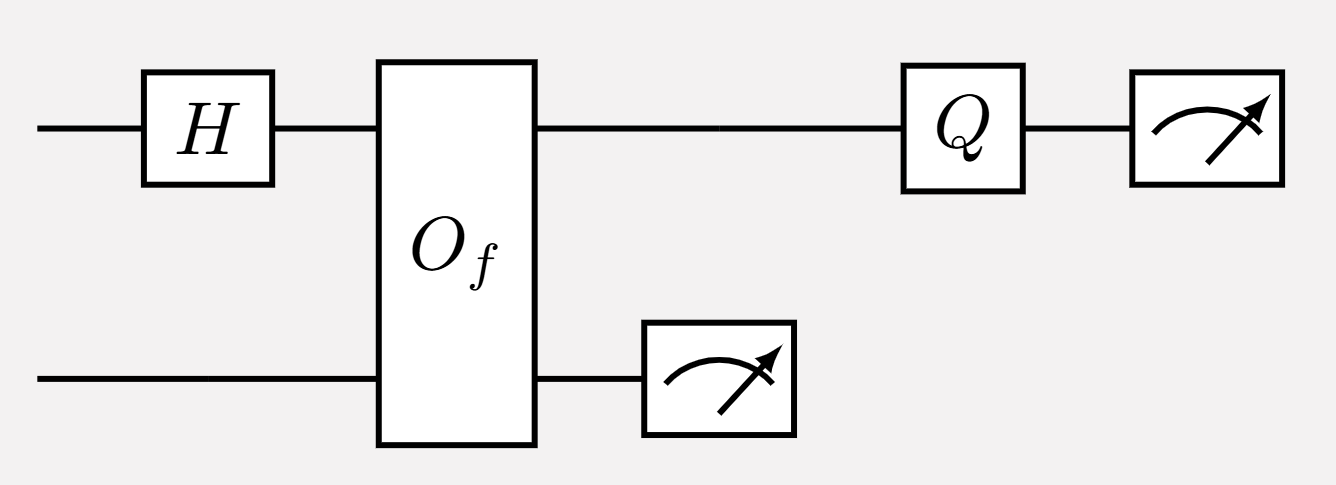
\includegraphics[width=0.5\textwidth]{img/shor_circuit.png}
		      \end{figure}
	\end{enumerate}
\end{greyframe}
Po kroku 4. na pierwszych \( n \) kubitach zostają tylko takie układy \( x \), dla których \( f(x) = y \) i~każdy z nich jest równie prawdopodobny.
Oznaczmy je przez
\[
	T = \set{x : 0 \leq x \leq N-1,\ f(x) = y}
\]
Na ostatnich \( n \) kubitach wykonujemy pomiar, otrzymując jakieś \( y \) i dalej te kubity nie są już potrzebne. Stan całego układu to:
\[
	\frac{1}{\sqrt{\abs{T}}} \sum_{x \in T} x \otimes y
\]
Załóżmy, że \( r \mid N \) i oznaczmy \( d = \frac{N}{r} \). Ze specyfiki funkcji \( f \) wynika, że istnieje takie \( s < r \), że \( T = \set{s, s + r, s + 2r, \ldots} \). Zatem \( \abs{T} = d \), czyli:
\[
	T = \set{s, s + r, s + 2r, \ldots, s + (d - 1)r}
\]
Na koniec, mając kubit w stanie
\[
	\frac{1}{\sqrt{d}} \sum_{x=0}^{N-1} b_x |x\rangle,
\]
gdzie \( b_x = \mathbbm{1}[x = s \!\!\pmod{r}] \), chcemy wyznaczyć \( r \) kwantową transformatą Fouriera.

\subsection*{Kwantowa transformata Fouriera}
Transformata Fouriera przekształca wektor \( v \) w wektor \( Q \cdot v \), gdzie \( Q \) jest macierzą Vandermonde'a:
\[
	Q = \frac{1}{\sqrt{N}} \begin{bmatrix}
		1      & 1            & 1               & \ldots & 1                   \\
		1      & \omega       & \omega^2        & \ldots & \omega^{N-1}        \\
		1      & \omega^2     & \omega^4        & \ldots & \omega^{2(N-1)}     \\
		1      & \omega^3     & \omega^6        & \ldots & \omega^{3(N-1)}     \\
		\vdots & \vdots       & \vdots          & \ddots & \vdots              \\
		1      & \omega^{N-1} & \omega^{2(N-1)} & \ldots & \omega^{(N-1)(N-1)}
	\end{bmatrix}
\]
Przeskalowanie przez \( \frac{1}{\sqrt{N}} \) jest potrzebne, żeby odwrotna transformata była taka sama czyli \\ \( Q \cdot \overline{Q^T} = I \).

Jako że \( Q \) jest unitarna, to możemy skonstruować bramkę Fouriera o \( n \) wejściach i \( n \) wyjściach, która mnoży \( n \) kubitów przez \( Q \).
Używamy do tego \( O(n^2) \) bramek \( H \) i \( R(\varphi) =
\brackets{\begin{smallmatrix}
		1 & 0 \\
		0 & e^{i\varphi}
	\end{smallmatrix}}
\).

Po przepuszczeniu kubitu
\[
	v = \frac{1}{\sqrt{d}} \sum_{x=0}^{N-1} b_x |x\rangle,
\]
przez bramkę \( Q \) otrzymujemy \( Q \cdot v = w = (w_1, \ldots, w_n) \), gdzie:
\[
	w_j = b_0 + b_1 \omega^j + b_2 \omega^{2j} + \ldots + b_{N-1} \omega^{(N-1)j},
\]
czyli, korzystając z tego, że \( b_x = \mathbbm{1}[x = s \!\!\pmod{r}] \), otrzymujemy:
\[
	w_j = \frac{1}{\sqrt{d}} \cdot \pars{ \omega^{s j} + \omega^{(s + r) j} + \ldots + \omega^{(s + (d - 1)r) j} } = \frac{1}{\sqrt{d}} \omega^{s j} \sum_{i = 0}^{d - 1} \omega^{i r j}.
\]
Jeśli \( N \mid r \cdot j \), to \( \omega^{r j} = 1 \), zatem
\[
	w_j = \sqrt{d} \cdot \omega^{s}
\]
Jeśli \( N \nmid r \cdot j \), to
\[
	w_j = \frac{1}{\sqrt{d}} \omega^{s} \cdot \frac{\omega^{r j d} - 1}{\omega^{r j} - 1} = \frac{1}{\sqrt{d}} \omega^{s} \cdot \frac{\omega^{j N} - 1}{\omega^{r j} - 1} = 0,
\]
Ponieważ \( N \mid r \cdot j \) wtedy i tylko wtedy, gdy \( d \mid j \), to wynikowym stanem jest:
\[
	\sqrt{d} \cdot \omega^s \cdot \sum_{d \mid x} |x\rangle
\]
A zatem kwantowa transformata Fouriera wykrywa okresowość.
Kubity w stanach: \[ s, s + r, s + 2r, \ldots \] po przejściu przez bramkę \( Q \) mogą mieć tylko stany: \[ d, 2d, 3d, \ldots, \] a przesunięcie \( s \) znika.

Mierząc taki kubit, dostajemy z równym prawdopodobieństem dowolny stan \( x \) taki, że \( d \mid x \). Na podstawie przypadkowego \( d = \frac{N}{r} \), chcemy poznać \( d \).
Powtarzamy więc cały algorytm kilkukrotnie -- za każdym razem dostajemy jakąś wielokrotność \( d \) (okres \( r \) jest taki sam, \( s \) może być inne).
Obliczając ich NWD, z dużym prawdopodobieństwem otrzymujemy \( d \).

W przypadku, kiedy \( r \nmid N \), po transformacie Fouriera i pomiarze możemy dostać każdy możliwy wynik. Jednak najbardziej prawdopodobne są te bliskie \( \frac{jN}{r} \) dla pewnego \( j \).
Ponieważ \( r \leq A \), to jeśli \( N > A^2 \), mając kilka pomiarów, też możemy odtworzyć \( r \).